\section{Simulation}
\markright{Simulation}

\begin{figure}[H]
  \centering
  \begin{subfigure}[b]{0.48\textwidth}
    \centering
    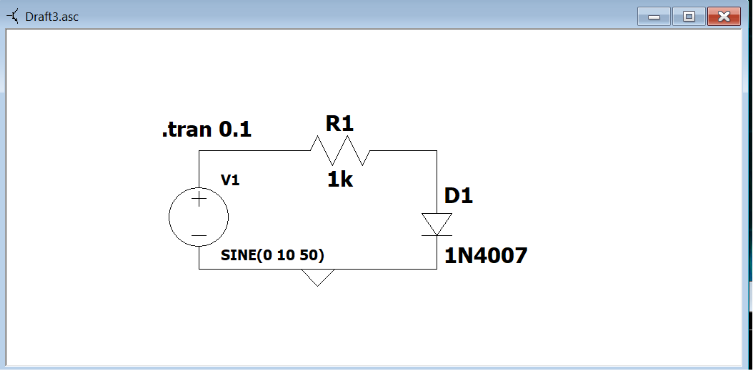
\includegraphics[width=\textwidth, height=4.5cm, keepaspectratio]{lab-03/assets/without-capacitor-schematic.png}
    \caption{Schematic}
  \end{subfigure}
  \hfill
  \begin{subfigure}[b]{0.48\textwidth}
    \centering
    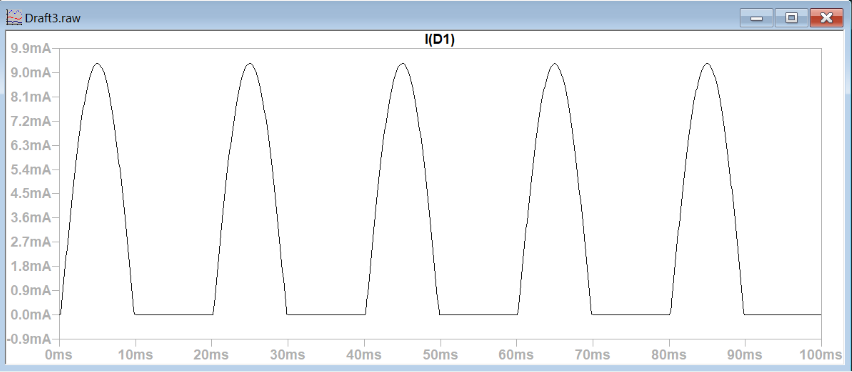
\includegraphics[width=\textwidth, height=4.5cm, keepaspectratio]{lab-03/assets/without-capacitor-output.png}
    \caption{Output}
  \end{subfigure}
  \caption{Simulation of Sinusoidal wave shape without capacitor: (a) Schematic and (b) Output.}
  \label{fig:lab03_sine}
\end{figure}

\begin{figure}[H]
  \centering
  \begin{subfigure}[b]{0.48\textwidth}
    \centering
    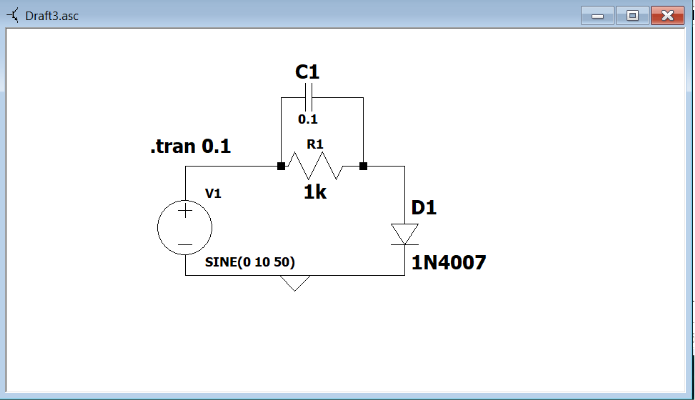
\includegraphics[width=\textwidth, height=4.5cm, keepaspectratio]{lab-03/assets/with-capacitor-schematic.png}
    \caption{Schematic}
  \end{subfigure}
  \hfill
  \begin{subfigure}[b]{0.48\textwidth}
    \centering
    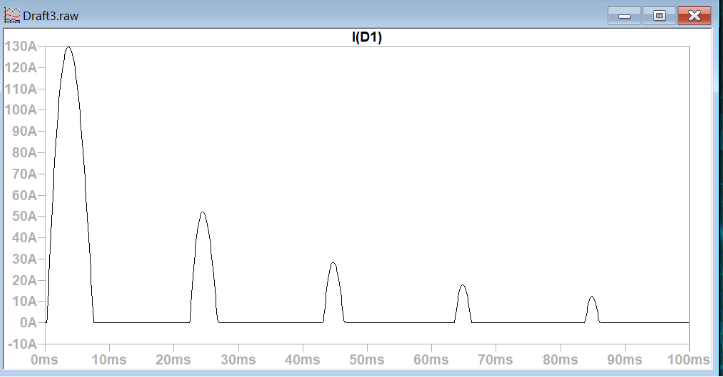
\includegraphics[width=\textwidth, height=4.5cm, keepaspectratio]{lab-03/assets/with-capacitor-output.png}
    \caption{Output}
  \end{subfigure}
  \caption{Simulation of Sinusoidal wave shape with capacitor: (a) Schematic and (b) Output.}
  \label{fig:lab03_sine}
\end{figure}
